\section{Recursos principals del bloc Persones}\label{sec:persons}

    \paragraph{}
    El centre d'aquest bloc de recursos és el recurs Persona. Aquest recurs, emmagatzema els detalls que identifiquen i caracteritzen a cada una de les persones de l'arbre, així com la informació bàsica sobre els seus relatius més propers.

    D'aquest recurs principal, pengen els enllaços cap als recursos que permeten obtenir informació sobre els relatius de la persona, els estudis realitzats sobre aquesta, l'historial de canvis, les fonts d'informació i les memòries afegides pels usuaris.

    La imatge~\ref{img:personsBloc} ofereix una visió de l'esquema que acabem de descriure i permet veure com el recurs Persona és enllaçat amb la resta de blocs que conformen l'arbre familiar.

    \begin{figure}[h]
        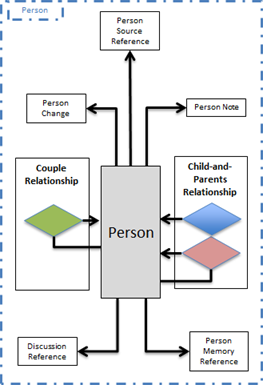
\includegraphics{05/03_personsCore}
        \centering
        \caption{El bloc de l'arbre familiar relatiu a les Persones.}\label{img:personsBloc}
    \end{figure}

    Aquest bloc de recursos és el més gran de tots i pràcticament emmagatzema tota la informació rellevant dels individus accessible a través de l'API. En els següents subapartats, s'exposaran els diferents recursos que conformen aquest bloc i quines són les peces d'informació utilitzables que contenen.

    Podreu observar, en les taules que representen l'estructura dels recursos, que a vegades, per la columna que marca el format de dades d'un paràmetre, aquest es troba especificat entre els caràcters `[' i `]'. Aquesta terminologia s'utilitza per indicar que aquest paràmetre és en realitat un recurs o objecte de dades diferent, inclòs dins del recurs estudiat.

    També s'observarà que sovint, els recursos exposats, hereten dades d'altres recursos i en els casos que aquests siguin rellevants, se n'exposarà l'estructura a l'apartat `Altres recursos interessants', més endavant en la memòria.

    \subsection{El recurs Persona (Person)}

    \paragraph{}
    El recurs Persona és el primer objecte amb què cal familiaritzar-se per tal de comprendre la potencialitat emmascarada d'aquesta API.

    Cada instància, fa referència a una persona diferent de l'arbre familiar i generalment, representa el punt d'entrada per tal d'accedir a tota la informació disponible sobre un individu, ja sigui perquè aquesta es troba inclosa en el recurs o esdevé accessible a través dels enllaços hypermedia.

    Els enllaços hypermedia del recurs Persona permeten accedir a la informació relativa als seus avantpassats, descendents, artefactes, historial de canvis, parelles, discussions, notes i fonts de dades.

    Les dades pròpies pel recurs Persona poden ser observades a la taula~\ref{tab:person}. Cal recordar que aquest recurs també hereta els paràmetres dels recursos Subjecte, Conclusió, Enllaços Hypermedia i Dades Extensibles que poden ser trobats a la secció `Altres recursos interessants'.

    \begin{center}
             \csvreader[
                separator=comma,
                before table=\sffamily\small,
                longtable={p{2cm-2\tabcolsep}p{3.5cm-2\tabcolsep}p{8.5cm-2\tabcolsep}},
                table head={\caption{Codificació GEDCOM X del recurs Persona}\label{tab:person}\\\toprule%
                    \headentry{m{2cm-2\tabcolsep}}{Paràmetre}
                    & \headentry{m{3.4cm-2\tabcolsep}}{Format de Dades}
                    & \headentry{m{8.5cm-2\tabcolsep}}{Descripció}\\\midrule},
                late after line=\\\midrule,
                late after last line=\\\bottomrule,
             ]
             {./tables/05/01_persons/person.csv}
             {param=\param,format=\format,desc=\desc}
             {\param&\format&\desc}
     \end{center}

    \subsection{El recurs Gènere (Gender)}

    \paragraph{}
    El recurs Gènere s'utilitza per especificar el gènere d'una persona en concret. Aquest recurs conté els paràmetres propis mostrats a la taula~\ref{tab:gender} i hereta els camps de dades dels recursos Conclusió, Enllaços Hypermedia i Dades Extensibles que poden ser trobats a la secció `Altres recursos interessants'.

    \begin{center}
             \csvreader[
                separator=comma,
                before table=\sffamily\small,
                longtable={p{2cm-2\tabcolsep}p{3.5cm-2\tabcolsep}p{8.5cm-2\tabcolsep}},
                table head={\caption{Codificació GEDCOM X del recurs Persona}\label{tab:gender}\\\toprule%
                    \headentry{m{2cm-2\tabcolsep}}{Paràmetre}
                    & \headentry{m{3.4cm-2\tabcolsep}}{Format de Dades}
                    & \headentry{m{8.5cm-2\tabcolsep}}{Descripció}\\\midrule},
                late after line=\\\midrule,
                late after last line=\\\bottomrule,
             ]
             {./tables/05/01_persons/gender.csv}
             {param=\param,format=\format,desc=\desc}
             {\param&\format&\desc}
     \end{center}


     \subsubsection{L'enumeració genderType}

     \paragraph{}
     L'enumeració genderType segueix l'estructura de definició GEDCOMX. Com a tal, els valors possibles per l'enumeració segueixen la pauta:

     http://gedcomx.org/ + `genderType'

     La següent taula mostra els tres possibles valors de l'enumeració genderType.

     \begin{center}
         \csvreader[
            no head,
            separator=comma,
            table head={\caption{Valors possibles per l'enumeració genderType}\label{tab:genderType}},
            before table=\sffamily\small,
            longtable={|p{3cm}|p{3cm}|p{3cm}|},
            column count=4,
            late after head=\\\hline,
            late after line=\\\hline,
            late after last line=\\\hline,
         ]
         {./tables/05/01_persons/genderType.csv}
         {1=\one,2=\two,3=\three}
         {\one&\two&\three}
     \end{center}

    \subsection{Els recursos Nom, Forma del Nom i Part del Nom (Name, NameForm, NamePart)}

    \paragraph{}
    Aquest conjunt de recursos s'utilitza per representar la informació relativa als noms d'una persona.  Contenen informació sobre si un nom és el preferit de cara a ser utilitzat com a nom principal, en quin moment la persona va adoptar aquest nom i diferents formes de representació.

    Resulta útil poder accedir a diferents noms d'una mateixa persona, per poder alternar, per exemple, entre el seu mot i el nom en el moment de naixement o defunció.

    El recurs Nom està format pels paràmetres mostrats a la taula~\ref{res:name} i hereta també els paràmetres dels recursos Conclusió, Enllaços Hypermedia i Dades Extensibles que poden ser trobats a la secció `Altres recursos interessants'.

    Per altre banda, els recursos Forma del Nom i Part del Nom, contenen els paràmetres mostrats a les taules~\ref{res:nameForm} i~\ref{res:namePart} respectivament i hereten els paràmetres del recurs Dades Extensibles descrit en l'apartat `Altres recursos interessants'.

    \begin{center}
             \csvreader[
                separator=semicolon,
                before table=\sffamily\small,
                longtable={p{2cm-2\tabcolsep}p{3.5cm-2\tabcolsep}p{8.5cm-2\tabcolsep}},
                table head={\caption{Paràmetres del recurs Nom}\label{res:name}\\\toprule%
                    \headentry{m{2cm-2\tabcolsep}}{Paràmetre}
                    & \headentry{m{3.4cm-2\tabcolsep}}{Format de Dades}
                    & \headentry{m{8.5cm-2\tabcolsep}}{Descripció}\\\midrule},
                late after line=\\\midrule,
                late after last line=\\\bottomrule,
             ]
             {./tables/05/01_persons/name.csv}
             {param=\param,format=\format,desc=\desc}
             {\param&\format&\desc}
     \end{center}

     \begin{center}
         \csvreader[
         separator=comma,
         before table=\sffamily\small,
         longtable={p{2cm-2\tabcolsep}p{3.5cm-2\tabcolsep}p{8.5cm-2\tabcolsep}},
         table head={\caption{Paràmetres del recurs Forma del Nom}\label{res:nameForm}\\\toprule%
         \headentry{m{2cm-2\tabcolsep}}{Paràmetre}
         & \headentry{m{3.4cm-2\tabcolsep}}{Format de Dades}
         & \headentry{m{8.5cm-2\tabcolsep}}{Descripció}\\\midrule},
         late after line=\\\midrule,
         late after last line=\\\bottomrule,
         ]
         {./tables/05/01_persons/nameForm.csv}
         {param=\param,format=\format,desc=\desc}
         {\param&\format&\desc}
     \end{center}

     \begin{center}
         \csvreader[
         separator=semicolon,
         before table=\sffamily\small,
         longtable={p{2cm-2\tabcolsep}p{3.5cm-2\tabcolsep}p{8.5cm-2\tabcolsep}},
         table head={\caption{Paràmetres del recurs Part del Nom}\label{res:namePart}\\\toprule%
         \headentry{m{2cm-2\tabcolsep}}{Paràmetre}
         & \headentry{m{3.4cm-2\tabcolsep}}{Format de Dades}
         & \headentry{m{8.5cm-2\tabcolsep}}{Descripció}\\\midrule},
         late after line=\\\midrule,
         late after last line=\\\bottomrule,
         ]
         {./tables/05/01_persons/namePart.csv}
         {param=\param,format=\format,desc=\desc}
         {\param&\format&\desc}
     \end{center}

     \subsubsection{L'enumeració nameType}

     \paragraph{}
     L'enumeració nameType segueix l'estructura de definició GEDCOMX. Com a tal, els valors possibles per l'enumeració segueixen la pauta:

     http://gedcomx.org/ + `nameType'

     La següent taula mostra els possibles valors de l'enumeració nameType.

     \begin{center}
         \csvreader[
            no head,
            separator=comma,
            table head={\caption{Valors possibles per l'enumeració nameType}\label{enum:nameType}},
            before table=\sffamily\small,
            longtable={|p{3cm}|p{3cm}|p{3cm}|p{3cm}|},
            column count=4,
            late after head=\\\hline,
            late after line=\\\hline,
            late after last line=\\\hline,
         ]
         {./tables/05/01_persons/nameType.csv}
         {1=\one,2=\two,3=\three,4=\four}
         {\one&\two&\three&\four}
     \end{center}


   \subsubsection{L'enumeració namePartType}

   \paragraph{}
   L'enumeració namePartType segueix l'estructura de definició GEDCOMX. Com a tal, els valors possibles per l'enumeració segueixen la pauta:

   http://gedcomx.org/ + `namePartType'

   La següent taula mostra els possibles valors de l'enumeració namePartType.

   \begin{center}
       \csvreader[
          no head,
          separator=comma,
          table head={\caption{Valors possibles per l'enumeració namePartType}\label{enum:namePartType}},
          before table=\sffamily\small,
          longtable={|p{3cm}|p{3cm}|p{3cm}|p{3cm}|},
          column count=4,
          late after head=\\\hline,
          late after line=\\\hline,
          late after last line=\\\hline,
       ]
       {./tables/05/01_persons/namePartType.csv}
       {1=\one,2=\two,3=\three,4=\four}
       {\one&\two&\three&\four}
   \end{center}

   El fet que es puguin configurar valors diferents per cada part del nom i diferents noms per la mateixa persona, cobra certa importància, ja que per exemple, en els baptismes del catolicisme, es solen utilitzar tres noms de pila diferents.

   Un altre exemple, potser encara més clar, del benefici d'utilitzar aquest conjunt de recursos per definir els noms d'una persona, resideix en les diferencies d'ús dels cognoms arreu del món. Per exemple, als Estats Units, les persones només tenen un cognom, mentre que a Espanya i altres països, en tenim dos. A més a més, en molts països europeus, el cognom d'una persona canvia segons el seu estat civil (solter, casat, vidu, etcètera) i per tant, existeix un clar benefici en poder emmagatzemar-ne més d'un.

    \subsection{El recurs Esdeveniment (Fact)}

    \paragraph{}
    El recurs Esdeveniment, tal com el seu nom indica, conté informació sobre un esdeveniment relacionat a la vida d'una persona o relació familiar. En concret, proporciona detalls sobre el tipus d'esdeveniment del quel es tracta, així com la data i localització on va succeir.

    Aquest recurs està format pels paràmetres mostrats a la taula~\ref{res:fact} i els paràmetres heretats dels recursos Conclusió, Enllaços Hypermedia i Dades Extensibles que poden ser trobats a la secció `Altres recursos interessants'.

    \begin{center}
             \csvreader[
                separator=semicolon,
                before table=\sffamily\small,
                longtable={p{2cm-2\tabcolsep}p{3.5cm-2\tabcolsep}p{8.5cm-2\tabcolsep}},
                table head={\caption{Paràmetres del recurs Esdeveniment}\label{res:fact}\\\toprule%
                    \headentry{m{2cm-2\tabcolsep}}{Paràmetre}
                    & \headentry{m{3.4cm-2\tabcolsep}}{Format de Dades}
                    & \headentry{m{8.5cm-2\tabcolsep}}{Descripció}\\\midrule},
                late after line=\\\midrule,
                late after last line=\\\bottomrule,
             ]
             {./tables/05/01_persons/fact.csv}
             {param=\param,format=\format,desc=\desc}
             {\param&\format&\desc}
     \end{center}


     \subsubsection{L'enumeració factType}

     \paragraph{}
     L'enumeració factType segueix l'estructura de definició GEDCOMX. Com a tal, els possibles valors per l'enumeració segueixen la pauta:

     http://gedcomx.org/ + `factType'

     La següent taula mostra els possibles valors de l'enumeració factType.

     \begin{center}
         \csvreader[
            no head,
            separator=comma,
            table head={\caption{Valors possibles per l'enumeració factType}\label{enum:factType}},
            before table=\sffamily\small,
            longtable={|p{3cm}|p{3cm}|p{3cm}|p{3cm}|},
            column count=4,
            late after head=\\\hline,
            late after line=\\\hline,
            late after last line=\\\hline,
         ]
         {./tables/05/01_persons/factType.csv}
         {1=\one,2=\two,3=\three,4=\four}
         {\one&\two&\three&\four}
     \end{center}

    \subsection{El recurs Data (Date)}

    \paragraph{}
    Aquest recurs conté la informació sobre les dates relacionades a alguna dada genealògica i diferents formats d'aquesta.

    En concret, emmagatzema la informació pròpia que es mostra a la taula~\ref{res:date} i hereta els paràmetres del recurs Dades Extensibles que pot ser trobar a la secció `Altres recursos interessants'.

    \begin{center}
             \csvreader[
                separator=comma,
                before table=\sffamily\small,
                longtable={p{2cm-2\tabcolsep}p{3.5cm-2\tabcolsep}p{8.5cm-2\tabcolsep}},
                table head={\caption{Paràmetres del recurs Data}\label{res:date}\\\toprule%
                    \headentry{m{2cm-2\tabcolsep}}{Paràmetre}
                    & \headentry{m{3.4cm-2\tabcolsep}}{Format de Dades}
                    & \headentry{m{8.5cm-2\tabcolsep}}{Descripció}\\\midrule},
                late after line=\\\midrule,
                late after last line=\\\bottomrule,
             ]
             {./tables/05/01_persons/date.csv}
             {param=\param,format=\format,desc=\desc}
             {\param&\format&\desc}
     \end{center}

    \subsection{El recurs Referència de localització (PlaceReference)}

    \paragraph{}
    Aquest recurs conté informació sobre localitzacions concretes vinculades a alguna dada genealògica.

    Aquest recurs conté les dades pròpies que es mostren a la taula~\ref{res:placeReference} i hereta també els paràmetres del recurs  Dades Extensibles que pot ser trobat a la secció `Altres recursos interessants'.

    \begin{center}
             \csvreader[
                separator=comma,
                before table=\sffamily\small,
                longtable={p{2cm-2\tabcolsep}p{3.5cm-2\tabcolsep}p{8.5cm-2\tabcolsep}},
                table head={\caption{Paràmetres del recurs Referència de localització}\label{res:placeReference}\\\toprule%
                    \headentry{m{2cm-2\tabcolsep}}{Paràmetre}
                    & \headentry{m{3.4cm-2\tabcolsep}}{Format de Dades}
                    & \headentry{m{8.5cm-2\tabcolsep}}{Descripció}\\\midrule},
                late after line=\\\midrule,
                late after last line=\\\bottomrule,
             ]
             {./tables/05/01_persons/placeReference.csv}
             {param=\param,format=\format,desc=\desc}
             {\param&\format&\desc}
     \end{center}

    \subsection{El recurs Descripció de Localització (PlaceDescription)}

    \paragraph{}
    Aquest recurs descriu els detalls d'una localització . Pretén representar la fotografia d'un lloc, en un moment específic de la història.

    A part dels paràmetres que seran descrits a continuació a la taula~\ref{res:placeDescription}, aquest recurs també hereta tots els paràmetres dels recursos Subjecte, Conclusió, Enllaços Hypermedia i Dades Extensibles que poden ser trobats a la secció `Altres recursos interessants'.

    \begin{center}
             \csvreader[
                separator=semicolon,
                before table=\sffamily\small,
                longtable={p{2cm-2\tabcolsep}p{3.5cm-2\tabcolsep}p{8.5cm-2\tabcolsep}},
                table head={\caption{Paràmetres del recurs Descripció de localització}\label{res:placeDescription}\\\toprule%
                    \headentry{m{2cm-2\tabcolsep}}{Paràmetre}
                    & \headentry{m{3.4cm-2\tabcolsep}}{Format de Dades}
                    & \headentry{m{8.5cm-2\tabcolsep}}{Descripció}\\\midrule},
                late after line=\\\midrule,
                late after last line=\\\bottomrule,
             ]
             {./tables/05/01_persons/placeDescription.csv}
             {param=\param,format=\format,desc=\desc}
             {\param&\format&\desc}
     \end{center}

    \subsection{El recurs Camps Bàsics (DisplayProperties)}

    \paragraph{}
    Aquest recurs conté el conjunt de propietats bàsiques d'una persona recopilades en un sol recurs. L'objectiu principal és facilitar l'accés a les dades més comunes per tal d'incrementar l'eficiència a l'hora de mostrar informació als usuaris i reduir així el nombre d'interaccions i connexions necessàries amb l'API.

    Com a extra, totes les propietats són localitzades amb l'idioma del local utilitzat.

    Les dades pròpies per aquest recurs s'indiquen a la taula~\ref{res:displayProperties} i el recurs també hereta les dades del recurs Dades Extensibles que pot ser trobat a la secció `Altres recursos interessants'.

    \begin{center}
             \csvreader[
                separator=comma,
                before table=\sffamily\small,
                longtable={p{2cm-2\tabcolsep}p{3.5cm-2\tabcolsep}p{8.5cm-2\tabcolsep}},
                table head={\caption{Paràmetres del recurs Camps Bàsics}\label{res:displayProperties}\\\toprule%
                    \headentry{m{2cm-2\tabcolsep}}{Paràmetre}
                    & \headentry{m{3.4cm-2\tabcolsep}}{Format de Dades}
                    & \headentry{m{8.5cm-2\tabcolsep}}{Descripció}\\\midrule},
                late after line=\\\midrule,
                late after last line=\\\bottomrule,
             ]
             {./tables/05/01_persons/displayProperties.csv}
             {param=\param,format=\format,desc=\desc}
             {\param&\format&\desc}
     \end{center}

    \subsection{El recurs Vista de Família (FamilyView)}

    \paragraph{}
    Aquest recurs conté informació bàsica sobre les relacions entre pares i fills. El recurs Relacions conté la informació canònica respecte a aquestes relacions i és el recurs que ha de ser utilitzat si es vol extreure més informació d'aquestes.

    Tanmateix, si només es desitja la informació bàsica de la relació, aquest recurs pot resultar molt convenient.

    Aquest recurs conté les dades pròpies que es mostren a la taula~\ref{res:familyView} i hereta també les dels recursos Enllaços Hypermedia i Dades Extensibles que poden ser trobades a la secció `Altres recursos interessants'.

    \begin{center}
             \csvreader[
                separator=comma,
                before table=\sffamily\small,
                longtable={p{2cm-2\tabcolsep}p{3.5cm-2\tabcolsep}p{8.5cm-2\tabcolsep}},
                table head={\caption{Paràmetres del recurs Vista de Família}\label{res:familyView}\\\toprule%
                    \headentry{m{2cm-2\tabcolsep}}{Paràmetre}
                    & \headentry{m{3.4cm-2\tabcolsep}}{Format de Dades}
                    & \headentry{m{8.5cm-2\tabcolsep}}{Descripció}\\\midrule},
                late after line=\\\midrule,
                late after last line=\\\bottomrule,
             ]
             {./tables/05/01_persons/familyView.csv}
             {param=\param,format=\format,desc=\desc}
             {\param&\format&\desc}
     \end{center}

